% Options for packages loaded elsewhere
\PassOptionsToPackage{unicode}{hyperref}
\PassOptionsToPackage{hyphens}{url}
\PassOptionsToPackage{dvipsnames,svgnames,x11names}{xcolor}
%
\documentclass[
  letterpaper,
  DIV=11,
  numbers=noendperiod]{scrreprt}

\usepackage{amsmath,amssymb}
\usepackage{iftex}
\ifPDFTeX
  \usepackage[T1]{fontenc}
  \usepackage[utf8]{inputenc}
  \usepackage{textcomp} % provide euro and other symbols
\else % if luatex or xetex
  \usepackage{unicode-math}
  \defaultfontfeatures{Scale=MatchLowercase}
  \defaultfontfeatures[\rmfamily]{Ligatures=TeX,Scale=1}
\fi
\usepackage{lmodern}
\ifPDFTeX\else  
    % xetex/luatex font selection
\fi
% Use upquote if available, for straight quotes in verbatim environments
\IfFileExists{upquote.sty}{\usepackage{upquote}}{}
\IfFileExists{microtype.sty}{% use microtype if available
  \usepackage[]{microtype}
  \UseMicrotypeSet[protrusion]{basicmath} % disable protrusion for tt fonts
}{}
\makeatletter
\@ifundefined{KOMAClassName}{% if non-KOMA class
  \IfFileExists{parskip.sty}{%
    \usepackage{parskip}
  }{% else
    \setlength{\parindent}{0pt}
    \setlength{\parskip}{6pt plus 2pt minus 1pt}}
}{% if KOMA class
  \KOMAoptions{parskip=half}}
\makeatother
\usepackage{xcolor}
\setlength{\emergencystretch}{3em} % prevent overfull lines
\setcounter{secnumdepth}{5}
% Make \paragraph and \subparagraph free-standing
\ifx\paragraph\undefined\else
  \let\oldparagraph\paragraph
  \renewcommand{\paragraph}[1]{\oldparagraph{#1}\mbox{}}
\fi
\ifx\subparagraph\undefined\else
  \let\oldsubparagraph\subparagraph
  \renewcommand{\subparagraph}[1]{\oldsubparagraph{#1}\mbox{}}
\fi

\usepackage{color}
\usepackage{fancyvrb}
\newcommand{\VerbBar}{|}
\newcommand{\VERB}{\Verb[commandchars=\\\{\}]}
\DefineVerbatimEnvironment{Highlighting}{Verbatim}{commandchars=\\\{\}}
% Add ',fontsize=\small' for more characters per line
\usepackage{framed}
\definecolor{shadecolor}{RGB}{241,243,245}
\newenvironment{Shaded}{\begin{snugshade}}{\end{snugshade}}
\newcommand{\AlertTok}[1]{\textcolor[rgb]{0.68,0.00,0.00}{#1}}
\newcommand{\AnnotationTok}[1]{\textcolor[rgb]{0.37,0.37,0.37}{#1}}
\newcommand{\AttributeTok}[1]{\textcolor[rgb]{0.40,0.45,0.13}{#1}}
\newcommand{\BaseNTok}[1]{\textcolor[rgb]{0.68,0.00,0.00}{#1}}
\newcommand{\BuiltInTok}[1]{\textcolor[rgb]{0.00,0.23,0.31}{#1}}
\newcommand{\CharTok}[1]{\textcolor[rgb]{0.13,0.47,0.30}{#1}}
\newcommand{\CommentTok}[1]{\textcolor[rgb]{0.37,0.37,0.37}{#1}}
\newcommand{\CommentVarTok}[1]{\textcolor[rgb]{0.37,0.37,0.37}{\textit{#1}}}
\newcommand{\ConstantTok}[1]{\textcolor[rgb]{0.56,0.35,0.01}{#1}}
\newcommand{\ControlFlowTok}[1]{\textcolor[rgb]{0.00,0.23,0.31}{#1}}
\newcommand{\DataTypeTok}[1]{\textcolor[rgb]{0.68,0.00,0.00}{#1}}
\newcommand{\DecValTok}[1]{\textcolor[rgb]{0.68,0.00,0.00}{#1}}
\newcommand{\DocumentationTok}[1]{\textcolor[rgb]{0.37,0.37,0.37}{\textit{#1}}}
\newcommand{\ErrorTok}[1]{\textcolor[rgb]{0.68,0.00,0.00}{#1}}
\newcommand{\ExtensionTok}[1]{\textcolor[rgb]{0.00,0.23,0.31}{#1}}
\newcommand{\FloatTok}[1]{\textcolor[rgb]{0.68,0.00,0.00}{#1}}
\newcommand{\FunctionTok}[1]{\textcolor[rgb]{0.28,0.35,0.67}{#1}}
\newcommand{\ImportTok}[1]{\textcolor[rgb]{0.00,0.46,0.62}{#1}}
\newcommand{\InformationTok}[1]{\textcolor[rgb]{0.37,0.37,0.37}{#1}}
\newcommand{\KeywordTok}[1]{\textcolor[rgb]{0.00,0.23,0.31}{#1}}
\newcommand{\NormalTok}[1]{\textcolor[rgb]{0.00,0.23,0.31}{#1}}
\newcommand{\OperatorTok}[1]{\textcolor[rgb]{0.37,0.37,0.37}{#1}}
\newcommand{\OtherTok}[1]{\textcolor[rgb]{0.00,0.23,0.31}{#1}}
\newcommand{\PreprocessorTok}[1]{\textcolor[rgb]{0.68,0.00,0.00}{#1}}
\newcommand{\RegionMarkerTok}[1]{\textcolor[rgb]{0.00,0.23,0.31}{#1}}
\newcommand{\SpecialCharTok}[1]{\textcolor[rgb]{0.37,0.37,0.37}{#1}}
\newcommand{\SpecialStringTok}[1]{\textcolor[rgb]{0.13,0.47,0.30}{#1}}
\newcommand{\StringTok}[1]{\textcolor[rgb]{0.13,0.47,0.30}{#1}}
\newcommand{\VariableTok}[1]{\textcolor[rgb]{0.07,0.07,0.07}{#1}}
\newcommand{\VerbatimStringTok}[1]{\textcolor[rgb]{0.13,0.47,0.30}{#1}}
\newcommand{\WarningTok}[1]{\textcolor[rgb]{0.37,0.37,0.37}{\textit{#1}}}

\providecommand{\tightlist}{%
  \setlength{\itemsep}{0pt}\setlength{\parskip}{0pt}}\usepackage{longtable,booktabs,array}
\usepackage{calc} % for calculating minipage widths
% Correct order of tables after \paragraph or \subparagraph
\usepackage{etoolbox}
\makeatletter
\patchcmd\longtable{\par}{\if@noskipsec\mbox{}\fi\par}{}{}
\makeatother
% Allow footnotes in longtable head/foot
\IfFileExists{footnotehyper.sty}{\usepackage{footnotehyper}}{\usepackage{footnote}}
\makesavenoteenv{longtable}
\usepackage{graphicx}
\makeatletter
\def\maxwidth{\ifdim\Gin@nat@width>\linewidth\linewidth\else\Gin@nat@width\fi}
\def\maxheight{\ifdim\Gin@nat@height>\textheight\textheight\else\Gin@nat@height\fi}
\makeatother
% Scale images if necessary, so that they will not overflow the page
% margins by default, and it is still possible to overwrite the defaults
% using explicit options in \includegraphics[width, height, ...]{}
\setkeys{Gin}{width=\maxwidth,height=\maxheight,keepaspectratio}
% Set default figure placement to htbp
\makeatletter
\def\fps@figure{htbp}
\makeatother

\KOMAoption{captions}{tableheading}
\makeatletter
\@ifpackageloaded{tcolorbox}{}{\usepackage[skins,breakable]{tcolorbox}}
\@ifpackageloaded{fontawesome5}{}{\usepackage{fontawesome5}}
\definecolor{quarto-callout-color}{HTML}{909090}
\definecolor{quarto-callout-note-color}{HTML}{0758E5}
\definecolor{quarto-callout-important-color}{HTML}{CC1914}
\definecolor{quarto-callout-warning-color}{HTML}{EB9113}
\definecolor{quarto-callout-tip-color}{HTML}{00A047}
\definecolor{quarto-callout-caution-color}{HTML}{FC5300}
\definecolor{quarto-callout-color-frame}{HTML}{acacac}
\definecolor{quarto-callout-note-color-frame}{HTML}{4582ec}
\definecolor{quarto-callout-important-color-frame}{HTML}{d9534f}
\definecolor{quarto-callout-warning-color-frame}{HTML}{f0ad4e}
\definecolor{quarto-callout-tip-color-frame}{HTML}{02b875}
\definecolor{quarto-callout-caution-color-frame}{HTML}{fd7e14}
\makeatother
\makeatletter
\@ifpackageloaded{bookmark}{}{\usepackage{bookmark}}
\makeatother
\makeatletter
\@ifpackageloaded{caption}{}{\usepackage{caption}}
\AtBeginDocument{%
\ifdefined\contentsname
  \renewcommand*\contentsname{Table of contents}
\else
  \newcommand\contentsname{Table of contents}
\fi
\ifdefined\listfigurename
  \renewcommand*\listfigurename{List of Figures}
\else
  \newcommand\listfigurename{List of Figures}
\fi
\ifdefined\listtablename
  \renewcommand*\listtablename{List of Tables}
\else
  \newcommand\listtablename{List of Tables}
\fi
\ifdefined\figurename
  \renewcommand*\figurename{Figure}
\else
  \newcommand\figurename{Figure}
\fi
\ifdefined\tablename
  \renewcommand*\tablename{Table}
\else
  \newcommand\tablename{Table}
\fi
}
\@ifpackageloaded{float}{}{\usepackage{float}}
\floatstyle{ruled}
\@ifundefined{c@chapter}{\newfloat{codelisting}{h}{lop}}{\newfloat{codelisting}{h}{lop}[chapter]}
\floatname{codelisting}{Listing}
\newcommand*\listoflistings{\listof{codelisting}{List of Listings}}
\makeatother
\makeatletter
\makeatother
\makeatletter
\@ifpackageloaded{caption}{}{\usepackage{caption}}
\@ifpackageloaded{subcaption}{}{\usepackage{subcaption}}
\makeatother
\ifLuaTeX
  \usepackage{selnolig}  % disable illegal ligatures
\fi
\usepackage{bookmark}

\IfFileExists{xurl.sty}{\usepackage{xurl}}{} % add URL line breaks if available
\urlstyle{same} % disable monospaced font for URLs
\hypersetup{
  pdftitle={Multilevel Multilingual},
  pdfauthor={Andrew Grogan-Kaylor},
  colorlinks=true,
  linkcolor={blue},
  filecolor={Maroon},
  citecolor={Blue},
  urlcolor={Blue},
  pdfcreator={LaTeX via pandoc}}

\title{Multilevel Multilingual}
\usepackage{etoolbox}
\makeatletter
\providecommand{\subtitle}[1]{% add subtitle to \maketitle
  \apptocmd{\@title}{\par {\large #1 \par}}{}{}
}
\makeatother
\subtitle{Multilevel Models in Stata, R and Julia}
\author{Andrew Grogan-Kaylor}
\date{2024-03-20}

\begin{document}
\maketitle

\renewcommand*\contentsname{Table of contents}
{
\hypersetup{linkcolor=}
\setcounter{tocdepth}{2}
\tableofcontents
}
\listoffigures
\listoftables
\bookmarksetup{startatroot}

\chapter{Multilevel Multilingual}\label{multilevel-multilingual}

\section{Introduction}\label{introduction}

Below, I describe the use of \href{https://www.stata.com/}{Stata},
\href{https://www.r-project.org/}{R}, and
\href{https://www.julialang.org/}{Julia} to estimate multilevel models.

\begin{tcolorbox}[enhanced jigsaw, opacityback=0, coltitle=black, colbacktitle=quarto-callout-tip-color!10!white, colframe=quarto-callout-tip-color-frame, opacitybacktitle=0.6, breakable, bottomtitle=1mm, toptitle=1mm, left=2mm, leftrule=.75mm, bottomrule=.15mm, rightrule=.15mm, arc=.35mm, title=\textcolor{quarto-callout-tip-color}{\faLightbulb}\hspace{0.5em}{Results Will Vary Slightly}, colback=white, titlerule=0mm, toprule=.15mm]

Estimating multilevel models is a complex endeavor. The details of how
this is accomplished are beyond the purview of this book. Suffice it to
say that across software packages there will be differences in
estimation routines, resulting in some numerical differences in the
results provided by different software packages. Substantively speaking,
however, results should agree across software.

\end{tcolorbox}

\section{The Data}\label{the-data}

The examples use the \texttt{simulated\_multilevel\_data.dta} file from
\href{https://agrogan1.github.io/multilevel-thinking/simulated-multi-country-data.html}{\emph{Multilevel
Thinking}}. Here is a
\href{https://github.com/agrogan1/multilevel-multilingual/raw/main/simulated_multilevel_data.dta}{direct
link} to download the data.

\begin{longtable}[]{@{}
  >{\centering\arraybackslash}p{(\columnwidth - 14\tabcolsep) * \real{0.1250}}
  >{\centering\arraybackslash}p{(\columnwidth - 14\tabcolsep) * \real{0.0750}}
  >{\centering\arraybackslash}p{(\columnwidth - 14\tabcolsep) * \real{0.1125}}
  >{\centering\arraybackslash}p{(\columnwidth - 14\tabcolsep) * \real{0.0750}}
  >{\centering\arraybackslash}p{(\columnwidth - 14\tabcolsep) * \real{0.1000}}
  >{\centering\arraybackslash}p{(\columnwidth - 14\tabcolsep) * \real{0.2750}}
  >{\centering\arraybackslash}p{(\columnwidth - 14\tabcolsep) * \real{0.1125}}
  >{\centering\arraybackslash}p{(\columnwidth - 14\tabcolsep) * \real{0.1250}}@{}}

\caption{\label{tbl-multilingual1}Sample of Simulated Multilevel Data}

\tabularnewline

\toprule\noalign{}
\begin{minipage}[b]{\linewidth}\centering
country
\end{minipage} & \begin{minipage}[b]{\linewidth}\centering
HDI
\end{minipage} & \begin{minipage}[b]{\linewidth}\centering
family
\end{minipage} & \begin{minipage}[b]{\linewidth}\centering
id
\end{minipage} & \begin{minipage}[b]{\linewidth}\centering
group
\end{minipage} & \begin{minipage}[b]{\linewidth}\centering
physical\_punishment
\end{minipage} & \begin{minipage}[b]{\linewidth}\centering
warmth
\end{minipage} & \begin{minipage}[b]{\linewidth}\centering
outcome
\end{minipage} \\
\midrule\noalign{}
\endhead
\bottomrule\noalign{}
\endlastfoot
1 & 69 & 1 & 1.1 & 2 & 2 & 3 & 59.18 \\
1 & 69 & 2 & 1.2 & 2 & 4 & 0 & 61.54 \\
1 & 69 & 3 & 1.3 & 1 & 4 & 4 & 51.87 \\
1 & 69 & 4 & 1.4 & 2 & 0 & 6 & 51.71 \\
1 & 69 & 5 & 1.5 & 2 & 3 & 2 & 55.88 \\
1 & 69 & 6 & 1.6 & 1 & 5 & 3 & 60.78 \\

\end{longtable}

\section{An Introduction To Equations and Syntax}\label{sec-syntax}

To explain statistical syntax for each software, I consider the general
case of a multilevel model with dependent variable \texttt{y},
independent variables \texttt{x} and \texttt{z}, clustering variable
\texttt{group}, and a random slope for \texttt{x}. \emph{i} is the index
for the person, while \emph{j} is the index for the \texttt{group}.

\begin{equation}\phantomsection\label{eq-MLMsimple}{y = \beta_0 + \beta_1 x_{ij} + \beta_2 z_{ij} + u_{0j} + u_{1j} \times x_{ij} + e_{ij}}\end{equation}

\subsection{Stata}

In Stata \texttt{mixed}, the syntax for a multilevel model of the form
described in Equation~\ref{eq-MLMsimple} is:

\begin{Shaded}
\begin{Highlighting}[]
\NormalTok{mixed }\FunctionTok{y}\NormalTok{ x || }\FunctionTok{group}\NormalTok{: x}
\end{Highlighting}
\end{Shaded}

\subsection{R}

In R \texttt{lme4}, the general syntax for a multilevel model of the
form described in Equation~\ref{eq-MLMsimple} is:

\begin{Shaded}
\begin{Highlighting}[]
\FunctionTok{library}\NormalTok{(lme4)}

\FunctionTok{lmer}\NormalTok{(y }\SpecialCharTok{\textasciitilde{}}\NormalTok{ x }\SpecialCharTok{+}\NormalTok{ z }\SpecialCharTok{+}\NormalTok{ (}\DecValTok{1} \SpecialCharTok{+}\NormalTok{ x }\SpecialCharTok{||}\NormalTok{ group), }\AttributeTok{data =}\NormalTok{ ...)}
\end{Highlighting}
\end{Shaded}

\subsection{Julia}

In Julia \texttt{MixedModels}, the general syntax for a multilevel model
of the form described in Equation~\ref{eq-MLMsimple} is:

\begin{Shaded}
\begin{Highlighting}[]
\ImportTok{using} \BuiltInTok{MixedModels}

\FunctionTok{fit}\NormalTok{(MixedModel, }\PreprocessorTok{@formula}\NormalTok{(y }\OperatorTok{\textasciitilde{}}\NormalTok{ x }\OperatorTok{+}\NormalTok{ z }\OperatorTok{+}\NormalTok{ (}\FloatTok{1} \OperatorTok{+}\NormalTok{ x }\OperatorTok{|}\NormalTok{ group)), data)}
\end{Highlighting}
\end{Shaded}

\bookmarksetup{startatroot}

\chapter{Descriptive Statistics}\label{descriptive-statistics}

\section{Descriptive Statistics}\label{descriptive-statistics-1}

\subsection{Stata}

\begin{Shaded}
\begin{Highlighting}[]

\KeywordTok{use}\NormalTok{ simulated\_multilevel\_data.dta }\CommentTok{// use data}
\end{Highlighting}
\end{Shaded}

We use \texttt{summarize} for \emph{continuous} variables, and
\texttt{tabulate} for \emph{categorical} variables.

\begin{Shaded}
\begin{Highlighting}[]

\KeywordTok{summarize}\NormalTok{ outcome warmth physical\_punishment HDI}

\KeywordTok{tabulate} \FunctionTok{group}
\end{Highlighting}
\end{Shaded}

\begin{verbatim}
    Variable |        Obs        Mean    Std. dev.       Min        Max
-------------+---------------------------------------------------------
     outcome |      3,000    53.46757     6.65179   33.39014   76.75101
      warmth |      3,000    3.524333    1.889956          0          7
physical_p~t |      3,000    2.494667    1.380075          0          5
         HDI |      3,000    64.76667    17.24562         33         87


  arbitrary |
      group |
   variable |      Freq.     Percent        Cum.
------------+-----------------------------------
          1 |      1,507       50.23       50.23
          2 |      1,493       49.77      100.00
------------+-----------------------------------
      Total |      3,000      100.00
\end{verbatim}

\subsection{R}

\begin{Shaded}
\begin{Highlighting}[]
\FunctionTok{library}\NormalTok{(haven) }\CommentTok{\# read data in Stata format}

\NormalTok{df }\OtherTok{\textless{}{-}} \FunctionTok{read\_dta}\NormalTok{(}\StringTok{"simulated\_multilevel\_data.dta"}\NormalTok{)}
\end{Highlighting}
\end{Shaded}

R's descriptive statistics functions rely heavily on whether a variable
is a \emph{numeric} variable, or a \emph{factor} variable. Below, I
convert two variables to factors (\texttt{factor}) before using
\texttt{summary}\footnote{\texttt{skimr} is an excellent new alternative
  library for generating descriptive statistics in R.} to generate
descriptive statistics.

\begin{Shaded}
\begin{Highlighting}[]
\NormalTok{df}\SpecialCharTok{$}\NormalTok{country }\OtherTok{\textless{}{-}} \FunctionTok{factor}\NormalTok{(df}\SpecialCharTok{$}\NormalTok{country)}

\NormalTok{df}\SpecialCharTok{$}\NormalTok{group }\OtherTok{\textless{}{-}} \FunctionTok{factor}\NormalTok{(df}\SpecialCharTok{$}\NormalTok{group)}

\FunctionTok{summary}\NormalTok{(df)}
\end{Highlighting}
\end{Shaded}

\begin{verbatim}
    country          HDI            family            id            group   
 1      : 100   Min.   :33.00   Min.   :  1.00   Length:3000        1:1507  
 2      : 100   1st Qu.:53.00   1st Qu.: 25.75   Class :character   2:1493  
 3      : 100   Median :70.00   Median : 50.50   Mode  :character           
 4      : 100   Mean   :64.77   Mean   : 50.50                              
 5      : 100   3rd Qu.:81.00   3rd Qu.: 75.25                              
 6      : 100   Max.   :87.00   Max.   :100.00                              
 (Other):2400                                                               
 physical_punishment     warmth         outcome     
 Min.   :0.000       Min.   :0.000   Min.   :33.39  
 1st Qu.:2.000       1st Qu.:2.000   1st Qu.:48.78  
 Median :3.000       Median :4.000   Median :53.64  
 Mean   :2.495       Mean   :3.524   Mean   :53.47  
 3rd Qu.:3.250       3rd Qu.:5.000   3rd Qu.:58.06  
 Max.   :5.000       Max.   :7.000   Max.   :76.75  
                                                    
\end{verbatim}

\subsection{Julia}

\begin{Shaded}
\begin{Highlighting}[]
\ImportTok{using} \BuiltInTok{Tables}\NormalTok{, }\BuiltInTok{MixedModels}\NormalTok{, }\BuiltInTok{MixedModelsExtras}\NormalTok{, }\BuiltInTok{StatFiles}\NormalTok{, }\BuiltInTok{DataFrames}\NormalTok{, }\BuiltInTok{CategoricalArrays}\NormalTok{, }\BuiltInTok{DataFramesMeta}

\NormalTok{df }\OperatorTok{=} \FunctionTok{DataFrame}\NormalTok{(}\FunctionTok{load}\NormalTok{(}\StringTok{"simulated\_multilevel\_data.dta"}\NormalTok{))}
\end{Highlighting}
\end{Shaded}

Similarly to R, Julia relies on the idea of \emph{variable type}. I use
\texttt{transform} to convert the appropriate variables to
\emph{categorical} variables.

\begin{Shaded}
\begin{Highlighting}[]
\PreprocessorTok{@transform}\NormalTok{!(df, }\OperatorTok{:}\NormalTok{country }\OperatorTok{=} \FunctionTok{categorical}\NormalTok{(}\OperatorTok{:}\NormalTok{country))}

\PreprocessorTok{@transform}\NormalTok{!(df, }\OperatorTok{:}\NormalTok{group }\OperatorTok{=} \FunctionTok{categorical}\NormalTok{(}\OperatorTok{:}\NormalTok{group))}
\end{Highlighting}
\end{Shaded}

\begin{Shaded}
\begin{Highlighting}[]

\FunctionTok{describe}\NormalTok{(df) }\CommentTok{\# descriptive statistics}
\end{Highlighting}
\end{Shaded}

\begin{verbatim}
8×7 DataFrame
 Row │ variable             mean     min      median   max     nmissing  eltyp ⋯
     │ Symbol               Union…   Any      Union…   Any     Int64     Union ⋯
─────┼──────────────────────────────────────────────────────────────────────────
   1 │ country                       1.0               30.0           0  Union ⋯
   2 │ HDI                  64.7667  33.0     70.0     87.0           0  Union
   3 │ family               50.5     1.0      50.5     100.0          0  Union
   4 │ id                            1.1               9.99           0  Union
   5 │ group                         1.0               2.0            0  Union ⋯
   6 │ physical_punishment  2.49467  0.0      3.0      5.0            0  Union
   7 │ warmth               3.52433  0.0      4.0      7.0            0  Union
   8 │ outcome              53.4676  33.3901  53.6426  76.751         0  Union
                                                                1 column omitted
\end{verbatim}

\bookmarksetup{startatroot}

\chapter{Unconditional Model}\label{unconditional-model}

An \emph{unconditional} multilevel model is a model with no independent
variables. One should always run an unconditional model as the first
step of a multilevel model in order to get a sense of the way that
variation is apportioned in the model across the different levels.

\section{The Equation}\label{the-equation}

\begin{equation}\phantomsection\label{eq-MLMunconditional}{\text{outcome}_{ij}= \beta_0 + u_{0j} + e_{ij}}\end{equation}

The Intraclass Correlation Coefficient (ICC) is given by:

\begin{equation}\phantomsection\label{eq-ICCunconditional}{\text{ICC} = \frac{var(u_{0j})}{var(u_{0j}) + var(e_{ij})}}\end{equation}

In a two level multilevel model, the ICC provides a measure of the
amount of variation attributable to Level 2.

\section{Run Models}\label{run-models}

\subsection{Stata}

\begin{Shaded}
\begin{Highlighting}[]

\KeywordTok{use}\NormalTok{ simulated\_multilevel\_data.dta }\CommentTok{// use data}
\end{Highlighting}
\end{Shaded}

\begin{Shaded}
\begin{Highlighting}[]

\NormalTok{mixed outcome || country: }\CommentTok{// unconditional model}
  
\end{Highlighting}
\end{Shaded}

\begin{verbatim}
Performing EM optimization ...

Performing gradient-based optimization: 
Iteration 0:  Log likelihood = -9856.1548  
Iteration 1:  Log likelihood = -9856.1548  

Computing standard errors ...

Mixed-effects ML regression                           Number of obs    = 3,000
Group variable: country                               Number of groups =    30
                                                      Obs per group:
                                                                   min =   100
                                                                   avg = 100.0
                                                                   max =   100
                                                      Wald chi2(0)     =     .
Log likelihood = -9856.1548                           Prob > chi2      =     .

------------------------------------------------------------------------------
     outcome | Coefficient  Std. err.      z    P>|z|     [95% conf. interval]
-------------+----------------------------------------------------------------
       _cons |   53.46757   .3539097   151.08   0.000     52.77392    54.16122
------------------------------------------------------------------------------

------------------------------------------------------------------------------
  Random-effects parameters  |   Estimate   Std. err.     [95% conf. interval]
-----------------------------+------------------------------------------------
country: Identity            |
                  var(_cons) |   3.348734   .9702594      1.897816    5.908906
-----------------------------+------------------------------------------------
               var(Residual) |   40.88284   1.060908       38.8555    43.01597
------------------------------------------------------------------------------
LR test vs. linear model: chibar2(01) = 169.64        Prob >= chibar2 = 0.0000
\end{verbatim}

\begin{Shaded}
\begin{Highlighting}[]
  
\KeywordTok{estat}\NormalTok{ icc }\CommentTok{// ICC}
\end{Highlighting}
\end{Shaded}

\begin{verbatim}
Intraclass correlation

------------------------------------------------------------------------------
                       Level |        ICC   Std. err.     [95% conf. interval]
-----------------------------+------------------------------------------------
                     country |   .0757091   .0203761      .0442419    .1265931
------------------------------------------------------------------------------
\end{verbatim}

\subsection{R}

\begin{Shaded}
\begin{Highlighting}[]
\FunctionTok{library}\NormalTok{(haven)}

\NormalTok{df }\OtherTok{\textless{}{-}} \FunctionTok{read\_dta}\NormalTok{(}\StringTok{"simulated\_multilevel\_data.dta"}\NormalTok{)}
\end{Highlighting}
\end{Shaded}

\begin{Shaded}
\begin{Highlighting}[]
\FunctionTok{library}\NormalTok{(lme4) }\CommentTok{\# estimate multilevel models}

\NormalTok{fit0 }\OtherTok{\textless{}{-}} \FunctionTok{lmer}\NormalTok{(outcome }\SpecialCharTok{\textasciitilde{}}\NormalTok{ (}\DecValTok{1} \SpecialCharTok{|}\NormalTok{ country),}
             \AttributeTok{data =}\NormalTok{ df) }\CommentTok{\# unconditional model}

\FunctionTok{summary}\NormalTok{(fit0)}
\end{Highlighting}
\end{Shaded}

\begin{verbatim}
Linear mixed model fit by REML ['lmerMod']
Formula: outcome ~ (1 | country)
   Data: df

REML criterion at convergence: 19712.5

Scaled residuals: 
     Min       1Q   Median       3Q      Max 
-2.97650 -0.68006  0.00936  0.67580  3.03510 

Random effects:
 Groups   Name        Variance Std.Dev.
 country  (Intercept)  3.478   1.865   
 Residual             40.883   6.394   
Number of obs: 3000, groups:  country, 30

Fixed effects:
            Estimate Std. Error t value
(Intercept)    53.47       0.36   148.5
\end{verbatim}

\begin{Shaded}
\begin{Highlighting}[]
\FunctionTok{library}\NormalTok{(performance)}

\NormalTok{performance}\SpecialCharTok{::}\FunctionTok{icc}\NormalTok{(fit0) }\CommentTok{\# ICC}
\end{Highlighting}
\end{Shaded}

\begin{verbatim}
# Intraclass Correlation Coefficient

    Adjusted ICC: 0.078
  Unadjusted ICC: 0.078
\end{verbatim}

\subsection{Julia}

\begin{Shaded}
\begin{Highlighting}[]
\ImportTok{using} \BuiltInTok{Tables}\NormalTok{, }\BuiltInTok{MixedModels}\NormalTok{, }\BuiltInTok{MixedModelsExtras}\NormalTok{, }
\BuiltInTok{StatFiles}\NormalTok{, }\BuiltInTok{DataFrames}\NormalTok{, }\BuiltInTok{CategoricalArrays}\NormalTok{, }\BuiltInTok{DataFramesMeta}

\NormalTok{df }\OperatorTok{=} \FunctionTok{DataFrame}\NormalTok{(}\FunctionTok{load}\NormalTok{(}\StringTok{"simulated\_multilevel\_data.dta"}\NormalTok{))}
\end{Highlighting}
\end{Shaded}

\begin{Shaded}
\begin{Highlighting}[]
\PreprocessorTok{@transform}\NormalTok{!(df, }\OperatorTok{:}\NormalTok{country }\OperatorTok{=} \FunctionTok{categorical}\NormalTok{(}\OperatorTok{:}\NormalTok{country))}
\end{Highlighting}
\end{Shaded}

\begin{Shaded}
\begin{Highlighting}[]

\NormalTok{m0 }\OperatorTok{=} \FunctionTok{fit}\NormalTok{(MixedModel, }
         \PreprocessorTok{@formula}\NormalTok{(outcome }\OperatorTok{\textasciitilde{}}\NormalTok{ (}\FloatTok{1} \OperatorTok{|}\NormalTok{ country)), df) }\CommentTok{\# unconditional model}
\end{Highlighting}
\end{Shaded}

\begin{verbatim}
Linear mixed model fit by maximum likelihood
 outcome ~ 1 + (1 | country)
   logLik   -2 logLik     AIC       AICc        BIC    
 -9856.1548 19712.3097 19718.3097 19718.3177 19736.3288

Variance components:
            Column   Variance Std.Dev.
country  (Intercept)   3.34871 1.82995
Residual              40.88285 6.39397
 Number of obs: 3000; levels of grouping factors: 30

  Fixed-effects parameters:
──────────────────────────────────────────────────
               Coef.  Std. Error       z  Pr(>|z|)
──────────────────────────────────────────────────
(Intercept)  53.4676    0.353908  151.08    <1e-99
──────────────────────────────────────────────────
\end{verbatim}

\begin{Shaded}
\begin{Highlighting}[]

\FunctionTok{icc}\NormalTok{(m0) }\CommentTok{\# ICC}
\end{Highlighting}
\end{Shaded}

\begin{verbatim}
0.07570852291396266
\end{verbatim}

\bookmarksetup{startatroot}

\chapter{Cross Sectional Model}\label{cross-sectional-model}

\section{The Equation}\label{the-equation-1}

Recall the general model of Equation~\ref{eq-MLMsimple}, and the syntax
outlined in Section~\ref{sec-syntax}. Below in
Equation~\ref{eq-MLMsubstantive}, we consider a more substantive
example.

\begin{equation}\phantomsection\label{eq-MLMsubstantive}{\text{outcome}_{ij}= \beta_0 + \beta_1 \text{warmth}_{ij} + \beta_2 \text{physical punishment}_{ij} + \\ \beta_3 \text{group}_{ij} + \beta_4 \text{HDI}_{ij} + \\ u_{0j} + u_{1j} \times \text{warmth}_{ij} + e_{ij}}\end{equation}

\section{Stata}

\subsection{Get The Data}\label{get-the-data}

\begin{Shaded}
\begin{Highlighting}[]

\KeywordTok{use}\NormalTok{ simulated\_multilevel\_data.dta}
\end{Highlighting}
\end{Shaded}

\subsection{Graph}\label{graph}

\begin{Shaded}
\begin{Highlighting}[]
\KeywordTok{twoway} \KeywordTok{scatter}\NormalTok{ outcome warmth, }\CommentTok{///}
  \BaseNTok{xtitle}\NormalTok{(}\StringTok{"warmth"}\NormalTok{) }\BaseNTok{ytitle}\NormalTok{(}\StringTok{"outcome"}\NormalTok{) }\CommentTok{///}
  \BaseNTok{title}\NormalTok{(}\StringTok{"Outcome by Parental Warmth"}\NormalTok{) }

\KeywordTok{quietly} \KeywordTok{graph} \KeywordTok{export} \KeywordTok{scatter}\NormalTok{.png, }\KeywordTok{replace}
\end{Highlighting}
\end{Shaded}

\begin{figure}

\centering{

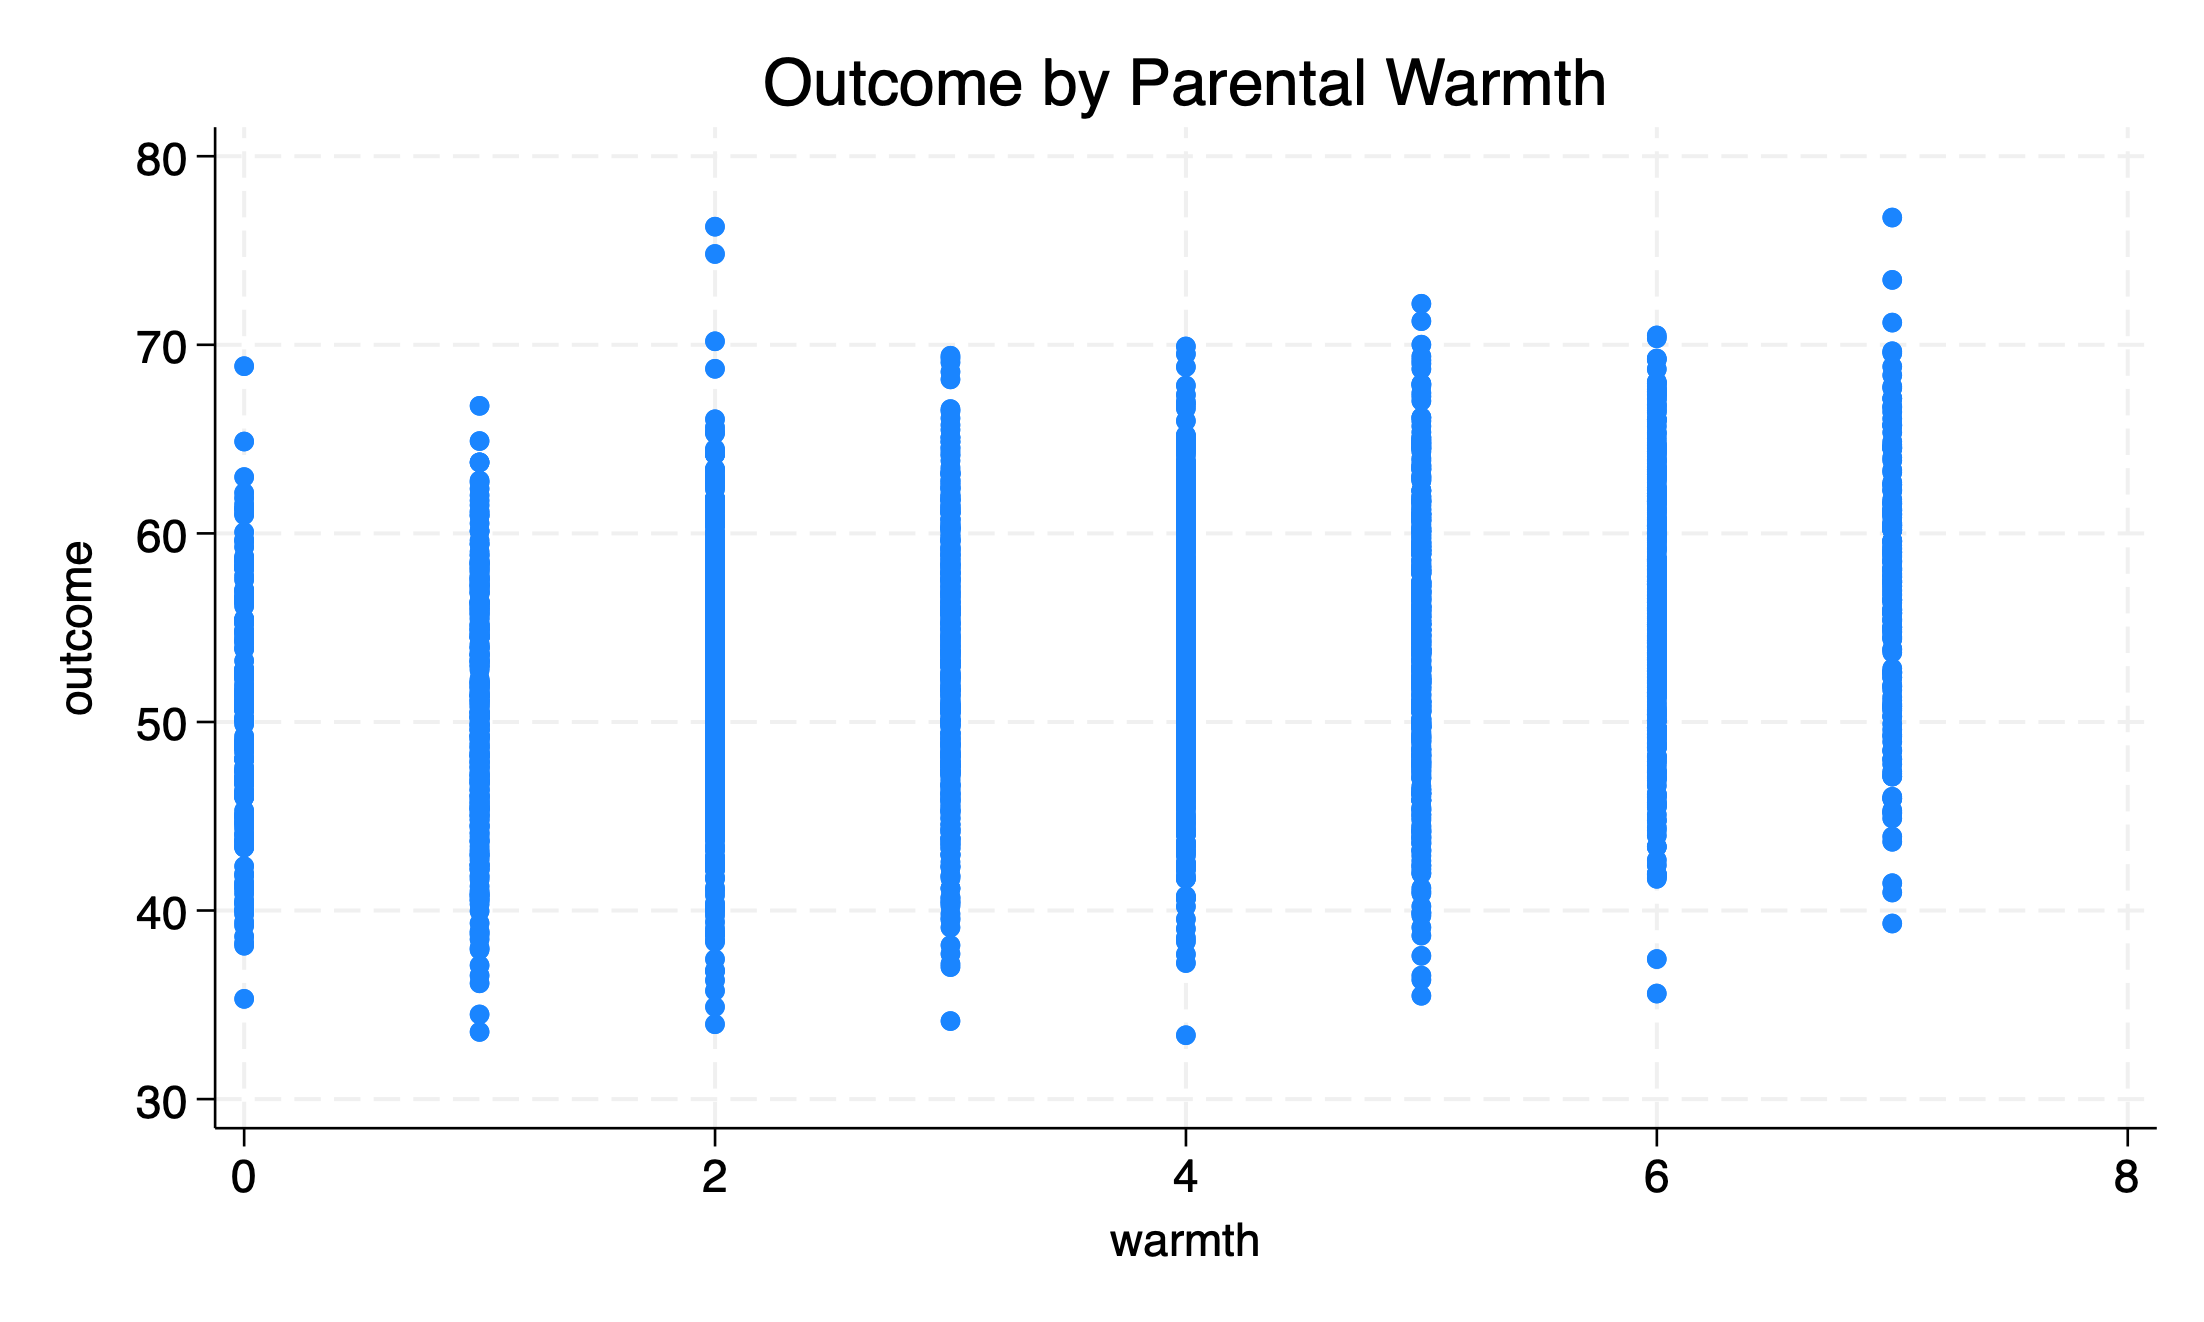
\includegraphics{scatter.png}

}

\caption{\label{fig-Stata}Outcome by Parental Warmth (Stata)}

\end{figure}%

\subsection{Run The Model}\label{run-the-model}

\begin{Shaded}
\begin{Highlighting}[]

\NormalTok{mixed outcome warmth physical\_punishment }\FunctionTok{group}\NormalTok{ HDI || country: warmth}
\end{Highlighting}
\end{Shaded}

\begin{verbatim}
Performing EM optimization ...

Performing gradient-based optimization: 
Iteration 0:  Log likelihood =  -9668.198  
Iteration 1:  Log likelihood = -9667.9551  
Iteration 2:  Log likelihood = -9667.9534  
Iteration 3:  Log likelihood = -9667.9533  
Iteration 4:  Log likelihood = -9667.9532  

Computing standard errors ...

Mixed-effects ML regression                          Number of obs    =  3,000
Group variable: country                              Number of groups =     30
                                                     Obs per group:
                                                                  min =    100
                                                                  avg =  100.0
                                                                  max =    100
                                                     Wald chi2(4)     = 401.26
Log likelihood = -9667.9532                          Prob > chi2      = 0.0000

-------------------------------------------------------------------------------------
            outcome | Coefficient  Std. err.      z    P>|z|     [95% conf. interval]
--------------------+----------------------------------------------------------------
             warmth |   .9616447   .0581825    16.53   0.000     .8476091     1.07568
physical_punishment |  -.8453802   .0798155   -10.59   0.000    -1.001816   -.6889448
              group |   1.084344   .2200539     4.93   0.000     .6530461    1.515642
                HDI |    .010557   .0204522     0.52   0.606    -.0295286    .0506426
              _cons |   49.87963   1.436612    34.72   0.000     47.06392    52.69534
-------------------------------------------------------------------------------------

------------------------------------------------------------------------------
  Random-effects parameters  |   Estimate   Std. err.     [95% conf. interval]
-----------------------------+------------------------------------------------
country: Independent         |
                 var(warmth) |   1.83e-06   .0000173      1.76e-14    190.9774
                  var(_cons) |   3.370262   .9633726      1.924651    5.901676
-----------------------------+------------------------------------------------
               var(Residual) |   36.01906   .9346936      34.23291    37.89842
------------------------------------------------------------------------------
LR test vs. linear model: chi2(2) = 198.01                Prob > chi2 = 0.0000

Note: LR test is conservative and provided only for reference.
\end{verbatim}

\section{R}

\subsection{Load The Needed Packages And Get The
Data}\label{load-the-needed-packages-and-get-the-data}

\begin{Shaded}
\begin{Highlighting}[]
\FunctionTok{library}\NormalTok{(haven)}

\NormalTok{df }\OtherTok{\textless{}{-}} \FunctionTok{read\_dta}\NormalTok{(}\StringTok{"simulated\_multilevel\_data.dta"}\NormalTok{)}
\end{Highlighting}
\end{Shaded}

\subsection{Graph}\label{graph-1}

\begin{Shaded}
\begin{Highlighting}[]
\FunctionTok{library}\NormalTok{(ggplot2)}

\FunctionTok{ggplot}\NormalTok{(df,}
       \FunctionTok{aes}\NormalTok{(}\AttributeTok{x =}\NormalTok{ warmth,}
           \AttributeTok{y =}\NormalTok{ outcome)) }\SpecialCharTok{+}
  \FunctionTok{geom\_point}\NormalTok{() }\SpecialCharTok{+}
  \FunctionTok{labs}\NormalTok{(}\AttributeTok{title =} \StringTok{"Outcome by Parental Warmth"}\NormalTok{)}
\end{Highlighting}
\end{Shaded}

\begin{figure}[H]

\centering{

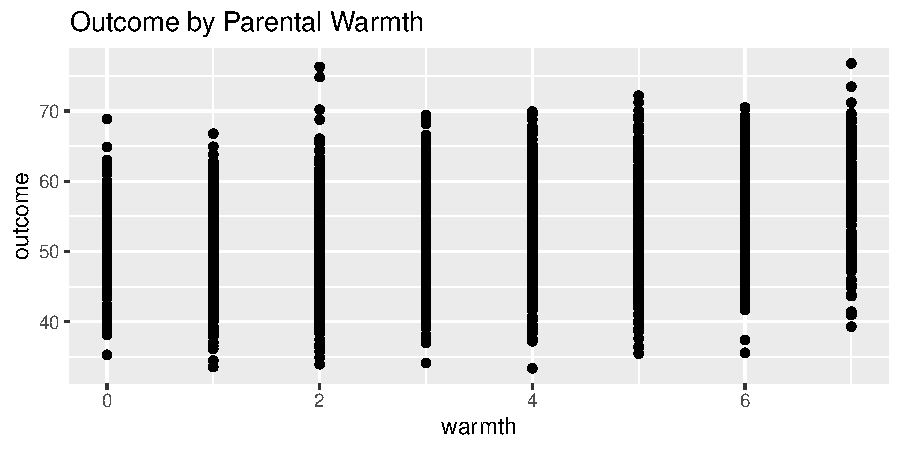
\includegraphics{cross-sectional-multilingual_files/figure-pdf/fig-R-1.pdf}

}

\caption{\label{fig-R}Outcome by Parental Warmth (R)}

\end{figure}%

\subsection{Run The Model}\label{run-the-model-1}

\begin{Shaded}
\begin{Highlighting}[]
\NormalTok{fit1 }\OtherTok{\textless{}{-}} \FunctionTok{lmer}\NormalTok{(outcome }\SpecialCharTok{\textasciitilde{}}\NormalTok{ warmth }\SpecialCharTok{+}\NormalTok{ physical\_punishment }\SpecialCharTok{+} 
\NormalTok{               group }\SpecialCharTok{+}\NormalTok{ HDI }\SpecialCharTok{+}
\NormalTok{               (}\DecValTok{1} \SpecialCharTok{+}\NormalTok{ warmth }\SpecialCharTok{||}\NormalTok{ country),}
             \AttributeTok{data =}\NormalTok{ df)}

\FunctionTok{summary}\NormalTok{(fit1)}
\end{Highlighting}
\end{Shaded}

\begin{verbatim}
Linear mixed model fit by REML ['lmerMod']
Formula: outcome ~ warmth + physical_punishment + group + HDI + ((1 |  
    country) + (0 + warmth | country))
   Data: df

REML criterion at convergence: 19350.3

Scaled residuals: 
    Min      1Q  Median      3Q     Max 
-3.4496 -0.6807  0.0016  0.6864  3.1792 

Random effects:
 Groups    Name        Variance  Std.Dev.
 country   (Intercept)  3.611568 1.90041 
 country.1 warmth       0.001876 0.04331 
 Residual              36.049124 6.00409 
Number of obs: 3000, groups:  country, 30

Fixed effects:
                    Estimate Std. Error t value
(Intercept)         49.88754    1.48203  33.662
warmth               0.96155    0.05875  16.367
physical_punishment -0.84556    0.07986 -10.588
group                1.08471    0.22017   4.927
HDI                  0.01044    0.02116   0.493

Correlation of Fixed Effects:
            (Intr) warmth physc_ group 
warmth      -0.126                     
physcl_pnsh -0.135 -0.025              
group       -0.218 -0.010 -0.019       
HDI         -0.925 -0.006  0.008 -0.001
\end{verbatim}

\section{Julia}

\subsection{Load The Needed Packages And Get The
Data}\label{load-the-needed-packages-and-get-the-data-1}

\begin{Shaded}
\begin{Highlighting}[]
\ImportTok{using} \BuiltInTok{Tables}\NormalTok{, }\BuiltInTok{MixedModels}\NormalTok{, }\BuiltInTok{StatFiles}\NormalTok{, }\BuiltInTok{DataFrames}\NormalTok{, }\BuiltInTok{CategoricalArrays}\NormalTok{, }\BuiltInTok{DataFramesMeta}

\NormalTok{df }\OperatorTok{=} \FunctionTok{DataFrame}\NormalTok{(}\FunctionTok{load}\NormalTok{(}\StringTok{"simulated\_multilevel\_data.dta"}\NormalTok{))}
\end{Highlighting}
\end{Shaded}

\subsection{Graph}\label{graph-2}

\begin{Shaded}
\begin{Highlighting}[]
\ImportTok{using} \BuiltInTok{StatsPlots}

\PreprocessorTok{@df}\NormalTok{ df }\FunctionTok{scatter}\NormalTok{(}\OperatorTok{:}\NormalTok{outcome, }\OperatorTok{:}\NormalTok{warmth, }
\NormalTok{               title }\OperatorTok{=} \StringTok{"Outcome by Parental Warmth"}\NormalTok{,}
\NormalTok{               ylabel }\OperatorTok{=} \StringTok{"outcome"}\NormalTok{,}
\NormalTok{               xlabel }\OperatorTok{=} \StringTok{"parental warmth"}\NormalTok{)}
\end{Highlighting}
\end{Shaded}

\begin{figure}[H]

\centering{

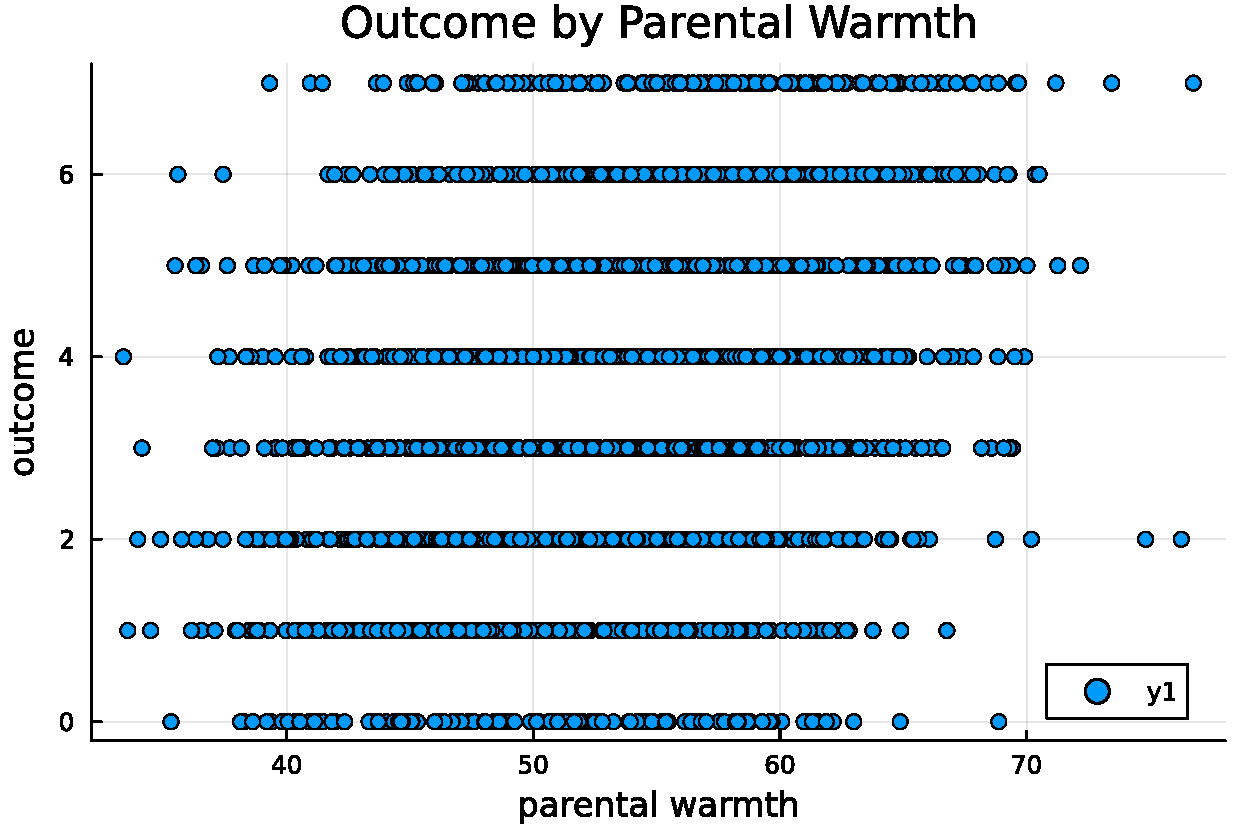
\includegraphics{cross-sectional-multilingual_files/figure-pdf/fig-Julia-J1.pdf}

}

\caption{\label{fig-Julia}Outcome by Parental Warmth (Julia)}

\end{figure}%

\subsection{Change Country To
Categorical}\label{change-country-to-categorical}

\begin{Shaded}
\begin{Highlighting}[]
\PreprocessorTok{@transform}\NormalTok{!(df, }\OperatorTok{:}\NormalTok{country }\OperatorTok{=} \FunctionTok{categorical}\NormalTok{(}\OperatorTok{:}\NormalTok{country))}
\end{Highlighting}
\end{Shaded}

\subsection{Run The Model}\label{run-the-model-2}

\begin{Shaded}
\begin{Highlighting}[]

\NormalTok{m1 }\OperatorTok{=} \FunctionTok{fit}\NormalTok{(MixedModel, }\PreprocessorTok{@formula}\NormalTok{(outcome }\OperatorTok{\textasciitilde{}}\NormalTok{ warmth }\OperatorTok{+}\NormalTok{ physical\_punishment }\OperatorTok{+} 
\NormalTok{               group }\OperatorTok{+}\NormalTok{ HDI }\OperatorTok{+}
\NormalTok{               (}\FloatTok{1} \OperatorTok{+}\NormalTok{ warmth }\OperatorTok{|}\NormalTok{ country)), df)}
\end{Highlighting}
\end{Shaded}

\begin{verbatim}
Linear mixed model fit by maximum likelihood
 outcome ~ 1 + warmth + physical_punishment + group + HDI + (1 + warmth | country)
   logLik   -2 logLik     AIC       AICc        BIC    
 -9667.9392 19335.8783 19353.8783 19353.9385 19407.9357

Variance components:
            Column    Variance   Std.Dev.   Corr.
country  (Intercept)   3.2369484 1.7991521
         warmth        0.0001080 0.0103903 +1.00
Residual              36.0187144 6.0015593
 Number of obs: 3000; levels of grouping factors: 30

  Fixed-effects parameters:
─────────────────────────────────────────────────────────────
                          Coef.  Std. Error       z  Pr(>|z|)
─────────────────────────────────────────────────────────────
(Intercept)          49.9018      1.43435     34.79    <1e-99
warmth                0.961545    0.0582135   16.52    <1e-60
physical_punishment  -0.845389    0.0798149  -10.59    <1e-25
group                 1.08524     0.220055     4.93    <1e-06
HDI                   0.0101984   0.0204401    0.50    0.6178
─────────────────────────────────────────────────────────────
\end{verbatim}



\end{document}
